\section{General Description}
\subsection{Introduction}

The control and measurement equipment along the Hall A beamline consists of 
various elements necessary to transport beam with the required specifications 
onto the reaction target and the dump and to simultaneously measure the 
properties of the beam relevant to the successful implementation of the 
physics program in Hall A.  The resolution and accuracy requirements in Hall 
A are such that special attention is paid to the following:

\vskip 0.5cm

1. Determination of the incident beam energy

2. Control of the beam position, direction, emittance and stability

3. Determination of the beam current, total charge and polarization.

\vskip 0.5cm
Table~\ref{tab:beam_tab1} gives a listing of all the various elements
along the Hall A beamline from the switch yard to the dump.
Figures~\ref{fig:Aline1},~\ref{fig:Aline2},~\ref{fig:Aline3} show
a schematic of the Hall A line starting at the shield wall.

\begin{figure}
\begin{center}
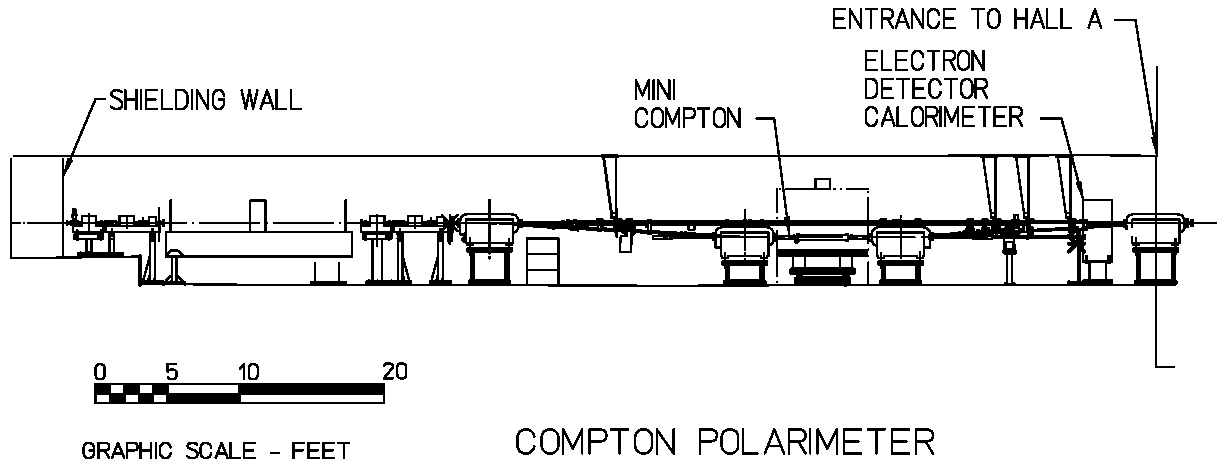
\includegraphics[angle=0,width=15cm]{compton_r}
{\linespread{1.}
\caption[Beamline: Hall A Beamline Overview]{Schematic of the Hall A beamline
starting at the shield wall to end of alcove.}
\label{fig:Aline1}}
\end{center}
\end{figure}

\begin{figure}
\begin{center}
\includegraphics[angle=0,width=15cm]{aline}
{\linespread{1.}
\caption[Beamline: Hall A Beamline Overview]{Schematic of the Hall A beamline
from the end of the alcove to the target chamber.}
\label{fig:Aline2}}
\end{center}
\end{figure}

\begin{figure}
\begin{center}
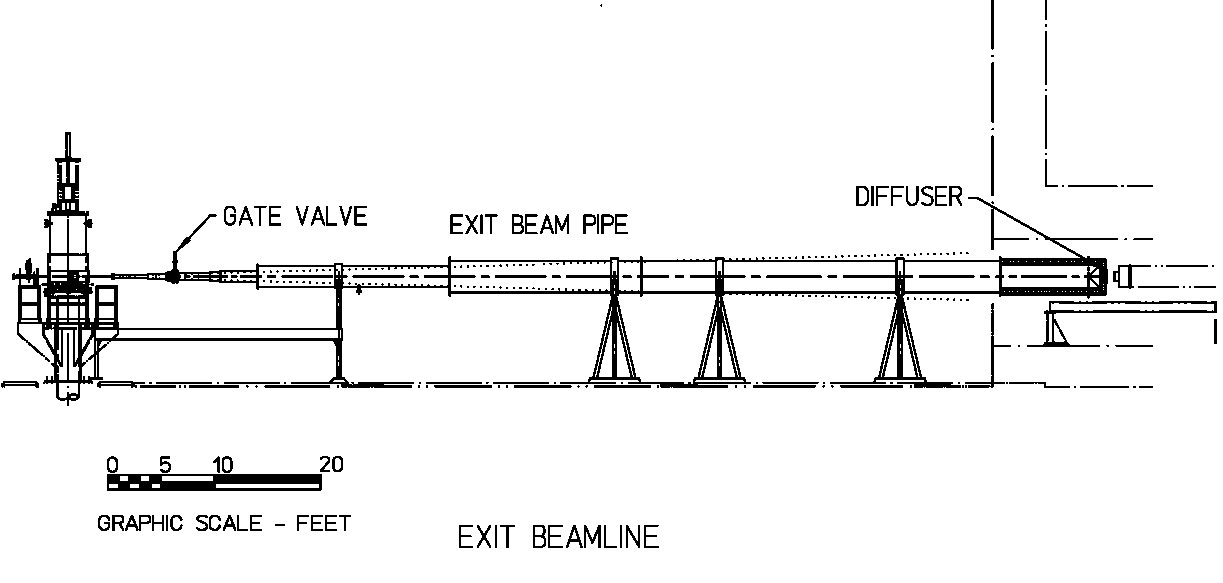
\includegraphics[angle=0,width=15cm]{dump_r}
{\linespread{1.}
\caption[Beamline: Hall A Beamline Overview]{Schematic of the Hall A beamline
from the target chamber to the dump diffuser.}
\label{fig:Aline3}}
\end{center}
\end{figure}
The basic Hall A beamline consists of the following:

\vskip 0.5cm
1. The Beam Entrance Channel

The beam entrance channel consists of stainless steel tubing connected with 
conflat type flanges. The usual opening is 2.5 inches for better vacuum 
conductance except through magnetic and beam diagnostic elements where it is 
usually 1 inch. Sections are isolated by vacuum valves and these are listed 
in Table~\ref{tab:beam_tab1}. Each section has a roughing port and is pumped with an ion pump. 
The pressure is about 10$^{-6}$ Torr. There are several sections along the 
beamline where users interface their equipment. Their individual systems 
are tested leak tight (to $ \le 10^{-9}$ Atm cm$^3$/sec).

\vskip 0.5cm
2. The Beam Optics Channel

These consist of dipoles, quadrupoles, sextupoles, and 
beam correctors with their 
standard girders and stands. Starting from the beam switchyard, there are 
eight dipoles in the arc section which (along with five  other smaller beam 
deflectors) bend the beam 37.5 degrees into the hall. Each dipole has a 
quadrupole and a pair of steering magnets (correctors) associated with it. 
After the shield wall at the entrance to the tunnel into the hall the beam is 
essentially undeflected onto the target and into the dump.  

The beamline optics elements are designed to deliver 
various optical tunes of the beam on to the physics target as well as 
simultaneously deliver various optical tunes at other locations along the 
beamline. These requirements are listed in Table~\ref{beam_tab3}. For the basic beamline we 
are able to deliver beam onto the hall A target in the achromatic
mode. 
 
\vskip 0.5cm
3. Beam Diagnostic Elements

These consist of beam position monitors (BPMs), beam current monitors,  wire 
scanners (superharps) and beam loss monitors. 
The wire scanners are fabricated by Saclay (French 
collaboration) and four have been installed along the beamline, two before 
the arc section and two after the arc section. They are essential for the 
beam energy determination by the arc method. Another two wire scanners are
installed on the bench just before the target to determine the beam 
position and direction of the beam at the target point with high precision 
and also measure the emmitance of the incident beam. They are also used to  
absolutely calibrate the two associated beam position monitors located  in 
front of the target. 


\vskip 0.5cm
4. Beam Exit Channel

After the target vacuum chamber, which was built by
the University of Virginia, there is an exit beam pipe which 
transfers the scattered beam onto the dump tunnel under vacuum. This exit beam 
pipe is made of a thin walled aluminum spiral corrugated pipe of welded 
construction. The largest diameter is 36 inches with a 0.164 inches wall 
thickness and the smallest diameter is 6 inches with a 0.042 inches wall 
thickness. The whole assembly is rather light (approximately 800 kg) and is 
supported by H shaped adjustable stands. To prevent possible linear collapse 
of the larger diameter sections under vacuum load, four aluminum channels of 
total cross-sectional area of 3'' are welded to its side. A vacuum of 
10$^{-5}$ Torr is maintained with a turbomolecular pump. The exit face of this 
pipe has a 12'' port and is connected to the diffuser with a Beryllium 
window.

\subsection{ Authorized Personnel}

All magnets (dipoles, quadrupoles, sextupoles, beam correctors) and beam 
diagnostic devices (BPMs, scanners, Beam Loss Monitor, viewers) necessary for 
the transport of the beam are controlled by Machine Control Center (MCC) 
through EPICS, except for special elements which are addressed in the 
subsequent sections. The detailed safety operational procedures for the Hall 
A beamline should be essentially the same as the one for the CEBAF machine 
and beamline. The Hall A staff liaison with the MCC are:

\begin{description}
\item[Primary Contact]A. Saha -x7605
\item[Secondary Contact]J.P. Chen -x7413
\end{description}

The Liaison between Accelerator Division and Physics Division is:

\begin{itemize}
\item[Liaison]H. Areti -x7187
\end{itemize}

\subsection{ Additional Safety Information}

Additional safety information is available in the following documents:

\begin{itemize}
\item[~] EH\&S Manual
\item[~] PSS Description Document (contact K. Mahoney for a copy)
\item[~] Accelerator Operations Directive (contact T. Oren for a copy)
\item[~] OSP - CEBAF Beam Operations (updated annually)
\end{itemize}

\subsection{ Machine/Beamline protection system}

The MPS system is composed of the fast shutdown system (FSD), beam loss 
monitor (BLM), and gun control system.

The FSD system is a network of permissive signals which terminate at the 
electron gun and chopper 1. The permissive to the gun and chopper
1 may be inhibited by any device connected to an FSD mode. Devices connected to the 
FSD system include vacuum valves, RF systems, Beam loss systems, beam current 
monitors, beam dumps, and particular to Hall A, the target motion mechanism 
and the raster (value and derivative).

The gun control system includes software program which monitors beam 
operating conditions and the state of the FSD and BLM systems. the program 
will warn the operators if a potential for beam damage exists. Potential for 
damage exists when running high average current beam, when FSD nodes are 
masked and when the beam power approaches the operating envelope limits for a 
specific beam dump.

\subsection{ Personnel Safety System}
 
Personnel safety system (PSS) console equipment is located in the main 
control room. It includes:

\begin{itemize}
\item[$\bullet$] Access control
\item[$\bullet$]Safety interlock
\item[$\bullet$]ODH monitoring
\item[$\bullet$]Radiation monitoring
\item[$\bullet$]Public address system.
\end{itemize}

\vspace*{0.5cm}
\begin{longtable}[hpt]{lllllr}

\hline
Girder & Diagnostic & Optics & Valves & Element & Distance (m) \\
\# & Elements & Elements & \& Pumps & \# & from target \\ \hline
\multicolumn{6}{c}{{\bf Beam Switch Yard}} \\ \hline 
& TV Viewer &&&ITV2C00 & 148.12862 \\ 
1CB2 & & Dipole (2.3m + & & MLA1C02 & 146.60000 \\
&&0.13m shim) &&& \\
1CB3 && BD && MBD1C00V & 144.18700 \\
&&&Valve & VBV1C00A & $\sim$142.78686 \\
& Current &&& SBC1C00 & $\sim$136.99564 \\
& Beam Stopper &&& SSS1C00 & $\sim$136.53844 \\
& Beam Stopper &&& SSS1C00A & $\sim$136.08124 \\
1C01 & BPM &&& IPM1C01 & 134.32465 \\
&& BC && MQA1C01 & 133.95000 \\
&&& Ion Pump & VIP1C01 & 133.04195 \\
1C02 & BPM &&& IPM1C02 & 132.02465 \\
&& BC && MQA1C02 & 131.65000 \\
&&&& MBC1C02V & 131.30685 \\
1C03 & BPM &&& IPM1C03 & 129.02465 \\
&& BC && MQA1C03 & 129.35000 \\
&&& Ion Pump & VIP1C03 & \\
&&& Rough Pump & VRV1C03 & 128.44195 \\
&&& Convectron & VTC1C03 & \\
1CB4 && Dipole (1m) && MBN1C04 & 116.70000 \\
1C04 & BPM &&& IPM1C04 & 115.42465 \\
&& Quad && MQA1C04 & 115.05000 \\
&& BC && MBC1C04H & 114.70685 \\
&&& Ion Pump & VIP1C04 & 114.14195 \\
1C05 & BPM &&& IPM1C05 & 112.12465 \\
&& Quad && MQA1C05 & 111.75000 \\
&& BC && MBC1C05V & 111.40685 \\
&&& Valve & VBV1C05A & \\
&&& Ion Pump & VIP1C05 & \\
&&& Rough Pump & VRV1C05 & 110.84195 \\
&&& Convectron & VTC1C05 & \\
1C06 &&& Valve & VBV1C06 & \\
& BPM &&& IPM1C06 & 104.82465 \\
&& Quad && MQA1C06 & 104.45000 \\
&& BC && MBC1C06H & 104.10685 \\
&&& Ion Pump & VIP1C06 & 103.54195 \\
1C07 & BPM &    &          & IPM1C07  & 99.52465 \\
     &     & BC &          & MBC1C07V & 98.61076 \\
     &     &    & Ion Pump & VIP1C07  & 98.24195 \\
\hline \multicolumn{6}{c}{{\bf Arc Section $\downarrow$}} \\ \hline 
1C08 & BPM &&& IPM1C08 & 93.42465 \\
&& Quad && MQA1C08 & 93.05000 \\
&& BC && MBC1C08H & 92.70685 \\
&& Sext && MSA1C08 & 92.40500 \\
& TV View &&& ITV1C08 & 92.21180 \\
&&& Ion Pump & VIP1C08 & \\
1CB5 && Dipole (3m) && MBA1C05 & 90.30000 \\
1C09 && Quad && MQA1C09 & 87.85000 \\
&& BC && MBC1C09H & 87.50685 \\
&& Sext && MSA1C09 & 87.20500 \\
1CB6 && Dipole (3m) && MBA1C06 & 85.10000 \\
1C10 & BPM &&& IPM1C10 & 83.02465 \\
&& Quad && MQA1C10 & 82.65000 \\
&& BC && MBC1C10H & 82.30685 \\
&& Sext && MSA1C10 & 82.00500 \\
&&& Ion Pump & VIP1C10 & 81.81180 \\
1CB7 && Dipole (3m) && MBA1C07 & 79.90000 \\
1C11 && Quad && MQA1C11 & 77.45000 \\
&& BC && MBC1C11V & 77.10685 \\
&& Sext && MSA1C11 & 76.80500 \\
&&& Covectron & VTC1C11 & 76.61180 \\
1CB8 && Dipole (3m) && MBA1C08 & 74.70000 \\
1C12 & BPM &&& IPM1C12 & 72.62465 \\
&& Quad && MQA1C12 & 72.25000 \\
&& BC && MBC1C12H & 71.90685 \\
&& Sext && MSA1C12 & 71.60500 \\
&&& Ion Pump & VIP1C12 & 71.41180 \\
1CB9 && Dipole (3m) && MBA1C09 & 69.50000 \\
1C13 && Quad && MQA1C13 & 67.05000 \\
&& BC && MBC1C13V & 66.70685 \\
&& Sext && MSA1C13 & 66.40500 \\
1CB10 && Dipole (3m) && MBA1C10 & 64.30000 \\
1C14 & BPM &&& IPM1C14 & 62.22465 \\
&& Quad && MQA1C14 & 61.85000 \\
&& BC && MBC1C14H & 61.50685 \\
&& Sext && MSA1C14 & 61.20500 \\
&&& Ion Pump & VIP1C14 & 61.01180 \\
1CB11 && Dipole (3m) && MBA1C11 & 59.10000 \\
1C15 &&& Valve & VBV1C15 & \\
&&& Rough Pump & VRV1C15 & \\
&& Quad && MQA1C15 & 56.65000 \\
&& BC && MBC1C15V & 56.30685 \\
&& Sect && MSA1C15 & 56.00500 \\
1CB12 && Dipole (3m) && MBA1C12 & 53.90000 \\ 
1C16 &&& Ion Pump & VIP1C16 & \\
&&& Convectron & VTC1C16 & \\
& BPM &&& IPM1C16 & 51.82465 \\
&& Quad && MQA1C16 & 51.45000 \\
&& BC && MBC1C16H & 51.10685 \\
&&& Valve & VBV1C16 & \\ 
\hline \multicolumn{6}{c}{{\bf Shield Wall $\rightarrow$ Hall A}} \\ \hline 
\multicolumn{5}{l}{SHIELD WALL(entrance surface)} & 50.70700 \\
\multicolumn{5}{l}{SHIELD WALL (exit surface)} &  49.651 \\
\hline
1C17 & TV Viewer &&& ITV1C17 & 49.411 \\
&& Quad && MQA1C17 & 49.100 \\
1C18 & BPM &&& IPM1C18 & 48.650 \\
&& Quad && MQA1C18 & 48.300 \\
&& BC && MBC1C18H & 47.957 \\
&& BC && MBC1C18V & 47.761 \\ \hline
%\noindent 
French & Scanner &&& IHA1C18A & 47.381 \\
Bench & Scanner &&& IHA1C18B & 43.673 \\ \hline
1C19 && Quad && MQA1C19 & 43.000 \\
1C20 & BPM &&& IPM1C120 & 42.550 \\
&& Quad && MQA1C20 & 42.200 \\
&& BC && MBC1C20H & 41.857 \\
&& BC && MBC1C20V & 41.661 \\
&&& Ion Pump & VIP1C20 & 41.450 \\ \hline
%\noindent  
\multicolumn{5}{l}{COMPTON Polarimeter Region} & 41.000 \\
& &&&& 25.500 \\
&&& Ion Pump & VIP1C20A & 34.500 \\
&&& Ion Pump & VIP1C20B & 29.500 \\ \hline
& Current &&& IBC1H00 & \\
&&&& IUN1H00 & 24.500 \\
&&&& IBC1H00A & \\
\multicolumn{2}{l}{Fast Raster} &&& MRA1H00H & 23.000 \\ 
&&&& MRA1H00H & \\ 
&&& Valve & VBV1H00 & 22.053 \\
\multicolumn{2}{l}{eP Energy Target} &&& VTP1H00A & 21.650 \\
&&& Ion Pump & VIP1H00A & 20.000 \\
1H01 &&& Valve & VBV1H01 & 19.020 \\
& TV View &&& ITV1H01 & 18.938 \\
& BPM &&& IPM1H01 & 18.650 \\
&& Quad && MQA1H01 & 18.300 \\
&& BC && MBC1H01H & 17.957 \\
&& BC && MBC1H01V & 17.761 \\ 
\hline
\multicolumn{2}{l}{Moller target} &&&& 17.5000 \\
1H02 && Quad && MQM1H02 & 16.500 \\
&&&& VRV1H02A \\
&&&& VTC1H02A \\
1H03 && Quad && MQO1H03 & 15.415 \\
1H03 && Quad && MQO1H03A & 14.758 \\
Moller && Dipole && MMA1H01 & 13.272 \\
&&& Ion Pump & VIP1H03A & 11.955 \\ \hline
Bench && BD && MBD1H03H & 8.132 \\
& BLM &&& IBC1H03A & 7.906 \\
&&& Valve & VBV1H03A & 7.786 \\
& BPM &&& IPM1H03A & 7.524 \\
& Scanner &&& IHA1H03A & 7.353 \\
&&& Ion Pump & VIP1H03B & 4.486 \\
&&&& VTC1H03A & \\
& BPM &&& IPM1H03B & 1.286 \\
& Scanner &&& IHA1H03B & 1.122 \\
&&& Valve & VBV1H03B & 0.953 \\ 
&&& Radiator & ERR1H & 0.726 \\ \hline
\multicolumn{4}{l}{TARGET TV Viewer} & ITV1H03A & 0.000 \\
\hline
\multicolumn{2}{l}{DUMP Face} &&&& -50.000 \\
\hline
\caption[Beamline: Hall A Beamline Elements]{Hall A beamline elements 
  from switchyard to Hall A beam dump (revised - 2/2/98)}
\label{tab:beam_tab1}
\end{longtable}


All distances are from the center of each element to the target (in 
meters).

\begin{table}[hp]
\vskip.25in
\begin{tabular}{|c|c|c|c|c|} \hline
{\bf Mode} & {\bf Spot Size} & {\bf Dispersion} & {\bf Position} & {\bf
Size} \\
& {\bf 4*$\sigma_{x,y}$} & {\bf $\eta$} & {\bf Stability} & {\bf
Stability} \\ \hline
Achromat & 140$\mu$m & 0 & 50$\mu$m & 50$\mu$m \\ \hline
Dispersive & $\propto \eta\delta$ & 4m to 12m & 50$\mu$m & 50$\mu$m \\
\hline
Defocussed & 0 to 3mm & 0 & $\pm$10\% & $\pm$10\% \\ \hline
\end{tabular}
\caption[Beamline: Optics Requirements Target]{ Line A Optics and Beam Requirements at Target}
\label{beam_tab3}
\end{table}

\begin{table}[ht]
\begin{tabular}{|c|c|c|c|c|} \hline
{\bf Mode} & {\bf Spot Size} & {\bf Dispersion} & {\bf Position} & {\bf
Size} \\
& {\bf 4*$\sigma_{x,y}$} & {\bf $\eta$} & {\bf Stability} & {\bf
Stability} \\ \hline
Energy-eP(d) & $>$100$\mu$m & 0 & 50$\mu$m & 50$\mu$m \\ \hline
Moller Pol. (d) & $>$250$\mu$m & 0 & 50$\mu$m & 50$\mu$m \\ \hline
Compton Pol.  & $>$80$\mu$m & 0 & 50$\mu$m & 50$\mu$m \\ \hline
*Energy-arc(d) && 15m & 50$\mu$m & 50$\mu$m \\ \hline
\end{tabular}
\caption[Beamline: Optics Requirements Other]{ Line A Optics and
Beam Requirements at Other Locations.}
\label{beam_tab4}
\vskip.25in
{\bf Notes:}
\begin{description}
\item[*] Build dispersion in arc section with all magnetic elements except
dipoles turned off.
\item[(d)] Destructive measurements.
\end{description}
\end{table}

\vfill\eject


% ===========  CVS info
% $Header: /group/halla/analysis/cvs/tex/osp/src/beamline/beam.tex,v 1.1 2003/06/05 17:28:32 gen Exp $
% $Id: beam.tex,v 1.1 2003/06/05 17:28:32 gen Exp $
% $Author: gen $
% $Date: 2003/06/05 17:28:32 $
% $Name:  $
% $Locker:  $
% $Log: beam.tex,v $
% Revision 1.1  2003/06/05 17:28:32  gen
% Initial revision
%
